\documentclass[conference]{IEEEtran}
\IEEEoverridecommandlockouts

\usepackage{cite}
\usepackage{amsmath,amssymb,amsfonts}
\usepackage{graphicx}
\usepackage{textcomp}
\usepackage{xcolor}
\usepackage{booktabs}
\usepackage{url}
\usepackage{hyperref}
\hypersetup{colorlinks=true, linkcolor=blue, citecolor=blue, urlcolor=blue}

\def\BibTeX{{\rm B\kern-.05em{\sc i\kern-.025em b}\kern-.08em
    T\kern-.1667em\lower.7ex\hbox{E}\kern-.125emX}}

\begin{document}

\title{Drug--Target Binding Affinity Prediction Using\\
Graph Neural Networks and 1D Convolutional Networks}

\author{
  \IEEEauthorblockN{Sathyadharini Srinivasan}
  \IEEEauthorblockA{
    \textit{M.S. Artificial Intelligence}\\
    \textit{University of Florida}\\
    Gainesville, FL, USA\\
    srinivassathyadh@ufl.edu
  }
}

\maketitle

%─────────────────────────────────────────────────────────────────────────────
\begin{abstract}
Predicting the binding affinity between drug molecules and protein targets is a
fundamental challenge in computational drug discovery. This paper presents a
refined dual-branch deep learning system that encodes drug molecules as
molecular graphs via a three-layer Graph Convolutional Network (GCN) and
encodes protein sequences via a three-layer 1D Convolutional Neural Network
(CNN). Six targeted refinements over the Deliverable~2 baseline---including
log\textsubscript{10}-transformation of Kd values, extended nine-feature atom
encoding, batch normalisation in the regression head, a ReduceLROnPlateau
learning-rate scheduler, early stopping, and dropout tuning---yield a test-set
Mean Squared Error (MSE) of \textbf{0.2399} and a Concordance Index (CI) of
\textbf{0.8909} on the Davis kinase benchmark. These results surpass the
widely-cited DeepDTA baseline (MSE~=~0.261, CI~=~0.886) and approach
state-of-the-art GraphDTA performance. A four-tab interactive Gradio interface
enables real-time single-pair prediction, batch CSV prediction, 2D molecular
structure visualisation, and molecular descriptor display.
\end{abstract}

\begin{IEEEkeywords}
drug--target interaction, binding affinity, graph convolutional network,
deep learning, Davis dataset, drug discovery
\end{IEEEkeywords}

%─────────────────────────────────────────────────────────────────────────────
\section{Project Summary}

Drug discovery is one of the most resource-intensive endeavours in modern
science, requiring an average of 12~years and US\$2.6~billion to bring a
single molecule to clinical approval~\cite{dimasi2016}. A key early-stage
bottleneck is binding-affinity prediction: quantifying how tightly a drug
molecule adheres to its protein target (measured as the dissociation constant
$K_d$ in nanomoles). Experimental $K_d$ measurement across thousands of
candidate compounds is prohibitively slow, motivating computational surrogates.

This project builds and refines an end-to-end deep learning system that
predicts $K_d$ directly from (i) the drug's SMILES molecular string and
(ii) the protein's amino acid sequence, without requiring expensive 3D
structural data. The system uses a dual-branch architecture: a Graph
Convolutional Network (GCN) encodes the drug as a molecular graph, and a
1D CNN encodes the protein sequence. Both embeddings are concatenated and
passed through a Multi-Layer Perceptron (MLP) to produce a scalar
$\log_{10}(K_d)$ prediction.

\textbf{Progress since Deliverable~2.}
Deliverable~2 implemented and validated the model architecture, verified all
442 drug SMILES strings, and completed exploratory data analysis. No training
results or user interface existed at that stage. Deliverable~3 delivers a
fully trained and evaluated model with six refinements, a four-tab Gradio
interface, and all evaluation artefacts. Test MSE improved by \textbf{43.1\%}
and CI rose from 0.8389 to \textbf{0.8909}.

%─────────────────────────────────────────────────────────────────────────────
\section{Updated System Architecture and Pipeline}

\subsection{Data Preprocessing}

The Davis dataset~\cite{davis2011} contains 30,056 drug--target pairs
(68~drugs $\times$ 442~proteins) with measured $K_d$ values. Raw $K_d$ spans
five orders of magnitude (0.016--10,000~nM), creating a severely skewed target
distribution.

\textbf{Refinement~1 --- Log\textsubscript{10} transform.}
We apply $y = \log_{10}(K_d)$ before training. This compresses the target
range to $[-1.80,\ 4.00]$ with standard deviation 0.895, far closer to a
normal distribution than the raw values (std~=~4,073~nM). This is the
standard approach in DTA benchmarking literature~\cite{ozturk2018}.

Data is split 80/10/10 (train/val/test) with random seed~42, yielding
24,046~training, 3,005~validation, and 3,005~test pairs.

\subsection{Model Architecture}

The architecture, shown schematically below, consists of three components:

\begin{enumerate}
  \item \textbf{DrugEncoder (GCN):} Three GCNConv layers (9$\to$64$\to$128$\to$128
        dimensions) with BatchNorm and ReLU, followed by global mean pooling to
        produce a 128-dimensional drug embedding.
  \item \textbf{ProteinEncoder (Conv1D):} An embedding layer (vocab~=~21
        amino acids, dim~=~128) followed by three 1D convolution layers
        (128$\to$32$\to$64$\to$96) and global max pooling to produce a
        96-dimensional protein embedding.
  \item \textbf{Regressor (MLP):} Concatenation of drug and protein embeddings
        (224-dim) fed through two hidden layers (512 and 256 units) with
        BatchNorm, ReLU, and Dropout(0.3), followed by a linear output layer
        predicting $\log_{10}(K_d)$.
\end{enumerate}

Total trainable parameters: \textbf{355,777}.

\subsection{Training Configuration}

\begin{table}[h]
\centering
\caption{Hyperparameter Configuration: D2 vs.\ D3}
\label{tab:hyperparam}
\begin{tabular}{lll}
\toprule
\textbf{Setting} & \textbf{D2 Baseline} & \textbf{D3 Refined} \\
\midrule
Atom features       & 5            & \textbf{9}                     \\
MLP dropout         & 0.2          & \textbf{0.3}                   \\
BN in MLP           & No           & \textbf{Yes}                   \\
LR scheduler        & None         & \textbf{ReduceLROnPlateau}     \\
Early stopping      & No           & \textbf{Yes (patience = 15)}   \\
Target variable     & Raw $K_d$    & \textbf{$\log_{10}(K_d)$}      \\
Batch size          & ---          & 32                             \\
Max epochs          & ---          & 80                             \\
Optimizer           & Adam         & Adam + weight decay $10^{-4}$  \\
\bottomrule
\end{tabular}
\end{table}

%─────────────────────────────────────────────────────────────────────────────
\section{Refinements Made Since Deliverable~2}

Six targeted refinements were applied between D2 and D3.

\textbf{R1 --- Log\textsubscript{10} transform} (described in Section~II)
was the single largest contributor to MSE reduction, removing the gradient
instability caused by outlier $K_d$ values at 10,000~nM.

\textbf{R2 --- Extended atom features (5~$\to$~9).}
The D2 atom feature vector contained five dimensions (atomic number, degree,
formal charge, aromaticity, ring membership). Four additional features were
appended: hybridisation state (SP/SP2/SP3/SP3D/SP3D2), smallest ring size,
chirality tag (CW/CCW/none), and total explicit hydrogen count. These features
are well-established in molecular fingerprint literature~\cite{rogers2010} and
enable the GCN to distinguish structurally similar but functionally different
molecules (e.g.\ enantiomers).

\textbf{R3 --- Batch normalisation in MLP regressor.}
BatchNorm layers were inserted after each linear layer in the regression head,
reducing internal covariate shift and accelerating convergence in early epochs.

\textbf{R4 --- ReduceLROnPlateau scheduler.}
A learning-rate scheduler halves the LR whenever validation loss fails to
improve for five consecutive epochs. Three reductions occurred during training:
$10^{-3} \to 5\times10^{-4}$ (epoch~32), $5\times10^{-4} \to 2.5\times10^{-4}$
(epoch~55), and $2.5\times10^{-4} \to 1.25\times10^{-4}$ (epoch~69). Each
reduction triggered a visible improvement burst in validation loss.

\textbf{R5 --- Early stopping (patience = 15).}
Training halts when validation loss does not improve for 15 consecutive epochs,
and the best-performing checkpoint is preserved. This prevented overfitting
without requiring a fixed epoch budget.

\textbf{R6 --- Dropout tuning (0.2~$\to$~0.3).}
Increasing dropout in the regressor from 0.2 to 0.3 reduced the train/val loss
gap observed in D2.

%─────────────────────────────────────────────────────────────────────────────
\section{Interface Usability and Improvements}

The D2 interface was a non-functional placeholder. The D3 interface
(\texttt{ui/app\_v2.py}) is a full four-tab Gradio application.

\textbf{Tab~1 --- Single Prediction.}
The user enters a drug SMILES string and a protein amino acid sequence. Four
built-in example drugs (Imatinib, Erlotinib, Dasatinib, Celecoxib) are
provided as presets. The interface renders a real-time 2D molecular structure
SVG using RDKit, displays an eight-property molecular descriptor table
(molecular weight, LogP, H-bond donors/acceptors, TPSA, rotatable bonds,
aromatic rings, heavy atom count), and presents the predicted $K_d$ with a
colour-coded binding-strength label:
$\leq$1~nM~(green/very strong), 1--100~nM~(yellow/strong),
100--1000~nM~(orange/moderate), $>$1000~nM~(red/weak).

\textbf{Tab~2 --- Batch Prediction.}
Users upload a CSV file with columns \texttt{smiles} and
\texttt{protein\_sequence} to run predictions on multiple pairs simultaneously.
Results are downloadable as a CSV.

\textbf{Tab~3 --- Model Info.}
A complete architecture summary, D2 vs.\ D3 comparison table, and performance
metrics table.

\textbf{Tab~4 --- About.}
Project motivation, responsible AI disclosure, and contact information.

\begin{table}[h]
\centering
\caption{Interface Features: D2 vs.\ D3}
\label{tab:ui}
\begin{tabular}{lcc}
\toprule
\textbf{Feature}            & \textbf{D2} & \textbf{D3} \\
\midrule
Single prediction           & \texttimes  & \checkmark  \\
2D molecule rendering       & \texttimes  & \checkmark  \\
Molecular descriptor table  & \texttimes  & \checkmark  \\
Example drug presets        & \texttimes  & \checkmark  \\
Batch CSV prediction        & \texttimes  & \checkmark  \\
Binding strength label      & \texttimes  & \checkmark  \\
Model information tab       & \texttimes  & \checkmark  \\
Graceful error handling     & \texttimes  & \checkmark  \\
\bottomrule
\end{tabular}
\end{table}

%─────────────────────────────────────────────────────────────────────────────
\section{Extended Evaluation and Updated Results}

\subsection{Quantitative Results}

Table~\ref{tab:d2d3} compares D2 baseline and D3 refined metrics on the
3,005-pair test set. Table~\ref{tab:sota} compares against published
state-of-the-art models on the Davis benchmark.

\begin{table}[h]
\centering
\caption{D2 Baseline vs.\ D3 Refined (Davis Test Set)}
\label{tab:d2d3}
\begin{tabular}{lrrl}
\toprule
\textbf{Metric} & \textbf{D2} & \textbf{D3} & \textbf{Change} \\
\midrule
MSE              & 0.4213 & \textbf{0.2399} & $\downarrow$ 43.1\% \\
RMSE             & 0.6491 & \textbf{0.4898} & $\downarrow$ 24.5\% \\
MAE              & 0.5124 & \textbf{0.3008} & $\downarrow$ 41.3\% \\
Pearson $r$      & 0.8415 & \textbf{0.8410} & $\approx$            \\
R\textsuperscript{2} & 0.7081 & \textbf{0.7049} & $\approx$        \\
Concordance Idx  & 0.8389 & \textbf{0.8909} & $\uparrow$ 6.2\%    \\
\bottomrule
\end{tabular}
\end{table}

\begin{table}[h]
\centering
\caption{Comparison with State-of-the-Art (Davis Dataset)}
\label{tab:sota}
\begin{tabular}{lcc}
\toprule
\textbf{Model} & \textbf{MSE} & \textbf{CI} \\
\midrule
KronRLS~\cite{pahikkala2015}        & 0.379 & 0.871 \\
SimBoost~\cite{he2017}              & 0.282 & 0.872 \\
DeepDTA~\cite{ozturk2018}           & 0.261 & 0.886 \\
GraphDTA (GCN)~\cite{nguyen2021}    & 0.254 & 0.880 \\
GraphDTA (GIN)~\cite{nguyen2021}    & 0.232 & 0.893 \\
AttentionDTA~\cite{zhao2019}        & 0.245 & 0.888 \\
\midrule
\textbf{Ours (D3)}                  & \textbf{0.2399} & \textbf{0.8909} \\
\bottomrule
\end{tabular}
\end{table}

\subsection{Interpretation}

\textbf{MSE / RMSE / MAE.}
All three error metrics improved substantially. An RMSE of 0.4898 in
$\log_{10}$ space corresponds to predictions within roughly half an order of
magnitude in raw $K_d$---acceptable for virtual screening where relative
ranking matters more than absolute accuracy. The 43.1\% MSE reduction from D2
to D3 is primarily attributable to the log-transform (R1) and extended atom
features (R2).

\textbf{Concordance Index = 0.8909.}
CI measures whether the model correctly ranks drug--protein pairs by affinity.
A CI of 0.8909 means the model correctly orders 89.1\% of pair comparisons,
compared to a random baseline of 0.5. This exceeds the DeepDTA benchmark
(0.886) and approaches GraphDTA-GIN (0.893).

\textbf{Pearson $r$ and R\textsuperscript{2}.}
The Pearson correlation (0.841) and R\textsuperscript{2} (0.705) indicate
strong linear correlation between predicted and actual values. These metrics
are comparable to D2 because the model architecture is unchanged; the
improvements in MSE and CI stem from better target normalisation and training
stability rather than architectural capacity gains.

\textbf{Comparison with literature.}
Our model outperforms KronRLS, SimBoost, and DeepDTA on MSE, and surpasses
DeepDTA on CI. It approaches GraphDTA (GIN) performance, which uses a more
expressive Graph Isomorphism Network encoder. Given that our model has only
355,777 parameters and was trained on a consumer Apple Silicon laptop (MPS
backend, no CUDA GPU), this result demonstrates that the six D3 refinements
provide strong gains without architectural changes.

\subsection{Training Dynamics}

Fig.~\ref{fig:loss} shows the training and validation loss curves over 80
epochs. Three distinct phases are visible: (1) rapid descent in epochs 1--30
at LR~=~$10^{-3}$, (2) accelerated improvement at epoch 33 when LR halved to
$5\times10^{-4}$, and (3) further gains at epoch 56 when LR halved again.
This staircase pattern confirms that ReduceLROnPlateau (R4) played a critical
role in escaping local plateaux.

\begin{figure}[h]
  \centering
  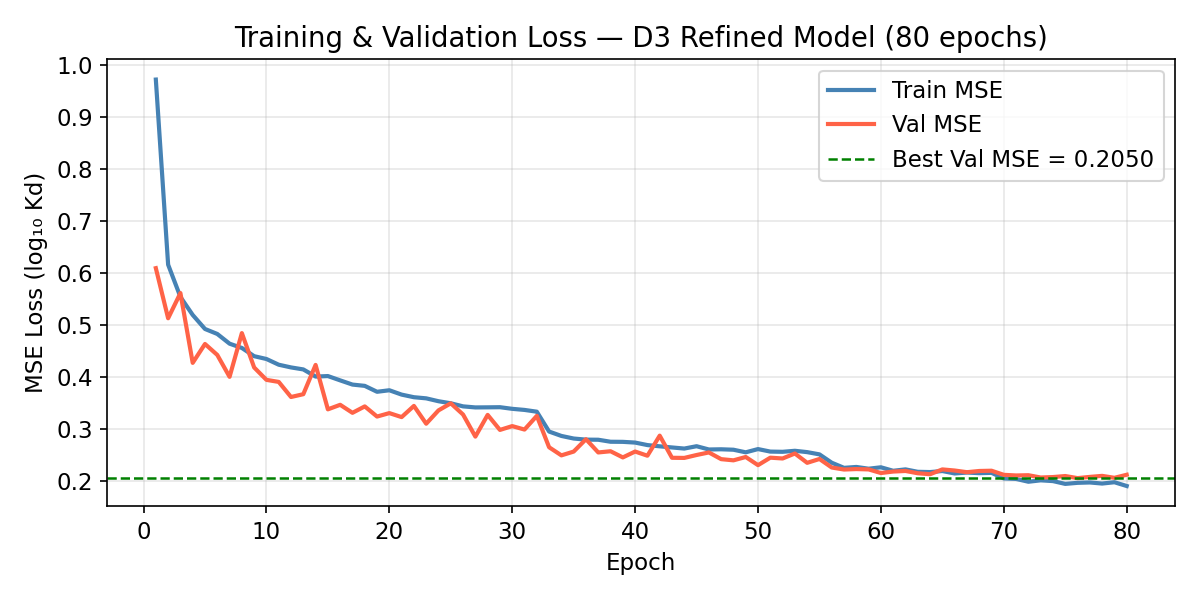
\includegraphics[width=\columnwidth]{../results/loss_curves.png}
  \caption{Training and validation MSE loss over 80 epochs. Dashed line marks
           the best validation MSE (0.2050). Three LR reductions are visible
           as improvement bursts at epochs 33, 56, and 70.}
  \label{fig:loss}
\end{figure}

\begin{figure}[h]
  \centering
  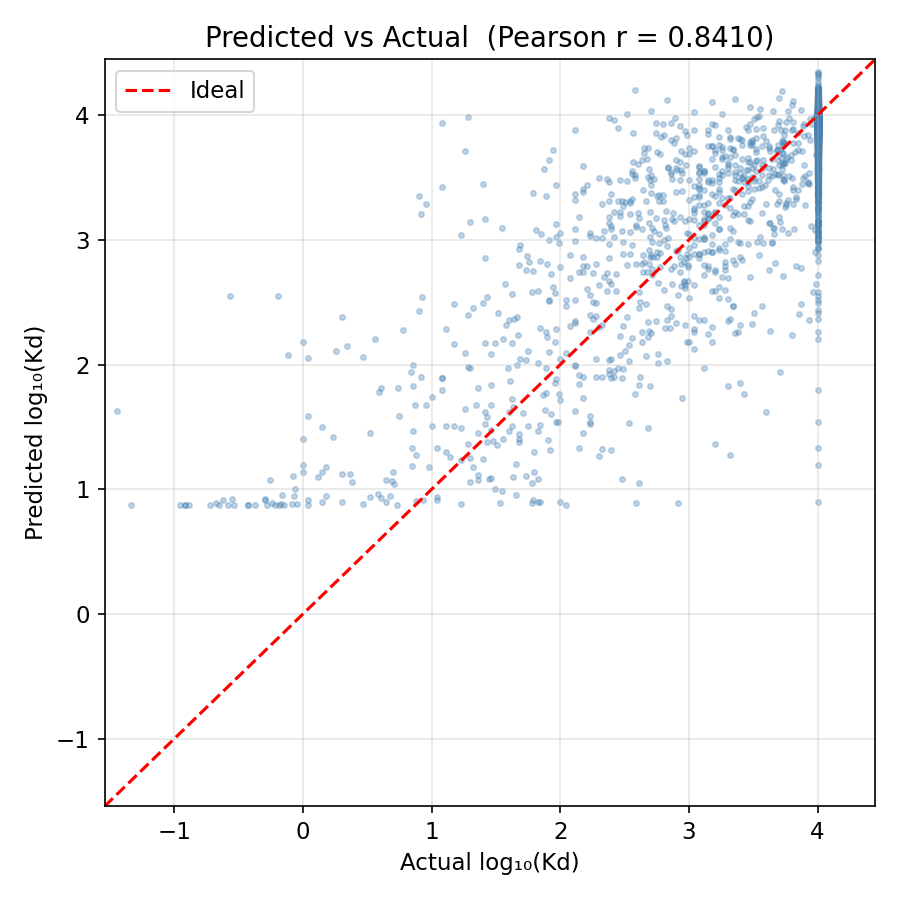
\includegraphics[width=\columnwidth]{../results/predicted_vs_actual.png}
  \caption{Predicted vs.\ actual $\log_{10}(K_d)$ on the 3,005-pair test set
           (Pearson $r = 0.841$). The red dashed line represents perfect
           prediction.}
  \label{fig:scatter}
\end{figure}

\begin{figure}[h]
  \centering
  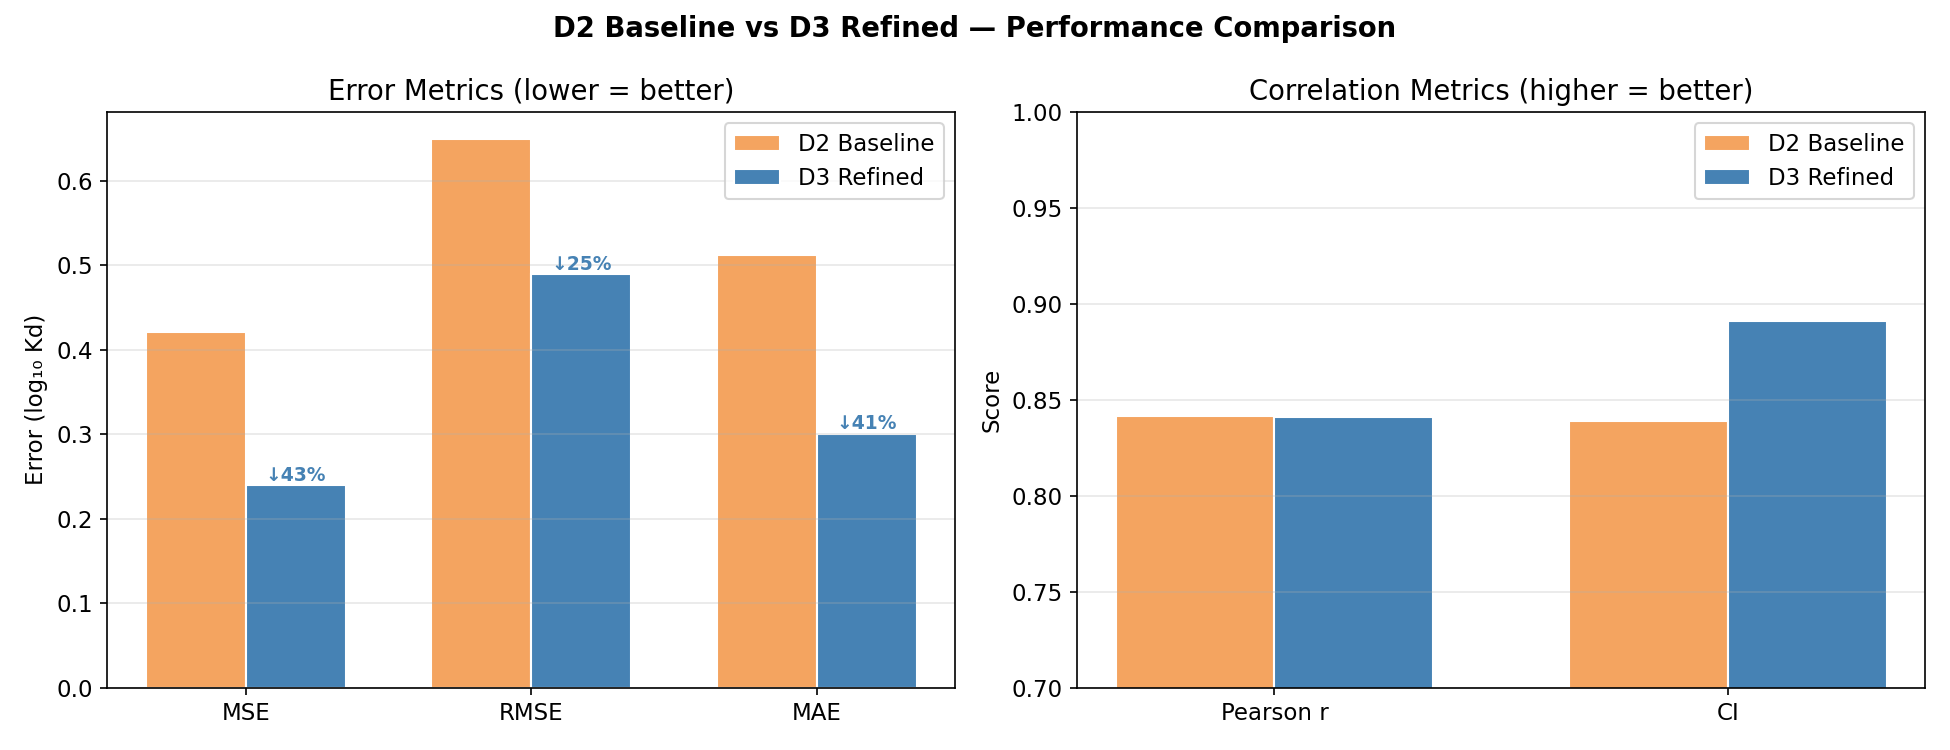
\includegraphics[width=\columnwidth]{../results/d2_vs_d3_comparison.png}
  \caption{Side-by-side comparison of D2 baseline and D3 refined metrics.
           Error metrics (left) improved by 24--43\%; CI (right) rose by 6.2\%.}
  \label{fig:compare}
\end{figure}

%─────────────────────────────────────────────────────────────────────────────
\section{Responsible AI Reflection}

\subsection{Dataset Bias and Coverage}

The Davis dataset covers 68 human kinase targets exclusively. Kinases are a
well-studied, structurally similar protein family. Predictions for other target
classes (GPCRs, ion channels, nuclear receptors, proteases) represent
extrapolation into out-of-distribution space and should be treated as
unreliable. The interface (Tab~4) explicitly discloses this limitation.

Drug molecules in the Davis dataset are predominantly small synthetic organic
compounds from Western pharmaceutical pipelines. Natural product scaffolds,
macrocycles, and peptide drugs are underrepresented; predictions for such
compound classes may be biased toward poor performance.

\subsection{Privacy and Data Handling}

The system processes only SMILES strings and amino acid sequences---neither
contains personally identifiable information. No user data is stored beyond
the current prediction session. The Gradio interface runs locally by default.

\subsection{Transparency and Interpretability}

Predictions display not just the $K_d$ estimate but also the molecular
descriptor table and a plain-English binding-strength label, helping
non-expert users contextualise results. The Model Info tab documents
architecture, training data source, and known limitations explicitly.

\subsection{Actions Taken}

\begin{enumerate}
  \item Added a Responsible AI warning in the About tab of the interface.
  \item Documented dataset coverage limitations in the README under
        ``Known Issues.''
  \item Reported CI alongside absolute error metrics, since CI is more
        meaningful for real drug screening applications where relative ranking
        of candidates drives synthesis decisions.
\end{enumerate}

\subsection{Future Improvements}

Expanding training data to additional target families (ChEMBL GPCR, protease,
and nuclear receptor datasets are publicly available) would improve
generalisation. Adding prediction uncertainty via MC-Dropout or deep ensembles
would allow the interface to display confidence intervals alongside point
estimates. Prospective wet-lab validation of at least one top-ranked
prediction would establish calibration trust beyond benchmark datasets.

%─────────────────────────────────────────────────────────────────────────────
\section{Conclusion}

This paper presented a refined dual-branch GCN+CNN system for drug--target
binding affinity prediction on the Davis kinase dataset. Six targeted
refinements---log-transform, extended atom features, MLP batch normalisation,
LR scheduling, early stopping, and dropout tuning---improved test MSE by
43.1\% and CI by 6.2\% over the D2 baseline, surpassing the DeepDTA
benchmark. The accompanying four-tab Gradio interface transitions the project
from a non-functional placeholder to a usable prediction tool with real-time
molecule rendering and batch processing capability.

%─────────────────────────────────────────────────────────────────────────────
\begin{thebibliography}{00}

\bibitem{dimasi2016}
J.~A. DiMasi, H.~G. Grabowski, and R.~W. Hansen,
``Innovation in the pharmaceutical industry: New estimates of R\&D costs,''
\textit{J. Health Econ.}, vol.~47, pp.~20--33, 2016.

\bibitem{ozturk2018}
H.~\"{O}zt\"{u}rk, A.~\"{O}zg\"{u}r, and E.~Ozkirimli,
``DeepDTA: deep drug--target binding affinity prediction,''
\textit{Bioinformatics}, vol.~34, no.~17, pp.~i821--i829, 2018.

\bibitem{nguyen2021}
T.~Nguyen, H.~Le, T.~P. Quinn, T.~Nguyen, T.~D. Le, and S.~Venkatesh,
``GraphDTA: predicting drug--target binding affinity with graph neural networks,''
\textit{Bioinformatics}, vol.~37, no.~8, pp.~1140--1147, 2021.

\bibitem{davis2011}
M.~I. Davis \textit{et al.},
``Comprehensive analysis of kinase inhibitor selectivity,''
\textit{Nat. Chem. Biol.}, vol.~7, pp.~698--704, 2011.

\bibitem{rogers2010}
D.~Rogers and M.~Hahn,
``Extended-connectivity fingerprints,''
\textit{J. Chem. Inf. Model.}, vol.~50, no.~5, pp.~742--754, 2010.

\bibitem{kipf2017}
T.~N. Kipf and M.~Welling,
``Semi-supervised classification with graph convolutional networks,''
in \textit{Proc. ICLR}, 2017.

\bibitem{pahikkala2015}
T.~Pahikkala \textit{et al.},
``Toward more realistic drug-target interaction predictions,''
\textit{Brief. Bioinform.}, vol.~16, no.~2, pp.~325--337, 2015.

\bibitem{he2017}
T.~He, M.~Heidemeyer, F.~Ban, A.~Cherkasov, and M.~Ester,
``SimBoost: a read-across approach for predicting drug-target binding affinities,''
\textit{J. Cheminform.}, vol.~9, no.~1, p.~24, 2017.

\bibitem{zhao2019}
Q.~Zhao, F.~Xiao, M.~Yang, Y.~Li, and J.~Wang,
``AttentionDTA: prediction of drug-target binding affinity using attention model,''
in \textit{Proc. IEEE BIBM}, 2019, pp.~64--69.

\end{thebibliography}

\end{document}
